%
% teil3.tex -- Beispiel-File für Teil 3
%
% (c) 2020 Prof Dr Andreas Müller, Hochschule Rapperswil
%
% !TEX root = ../../buch.tex
% !TEX encoding = UTF-8
%
\subsection{Kreuzung
\label{buch:paper:varalg:subsection:crossover}}
\index{Kreuzung}%
In diesem Schritt des Algorithmus werden aus den gewählten Elternpaaren 
neue Nachkommen erzeugt. Dies wird erreicht, indem Teile des genetischen 
Strings miteinander ausgetauscht werden, 
wie in der Abbildung \ref{fig:one_point_crossover} veranschaulicht.
Durch diesen Mechanismus wird die Variation aufrechterhalten. Wichtig ist es,
dass aus zwei Eltern immer genau zwei Nachkommen erzeugt werden. Würde
die Population wachsen, würde der Aufwand zwischen den Generationen
wachsen, was den Zweck des Algorithmus verfehlt. Daher muss die Grösse der
Population immer konstant bleiben.
\begin{figure}
	\centering
	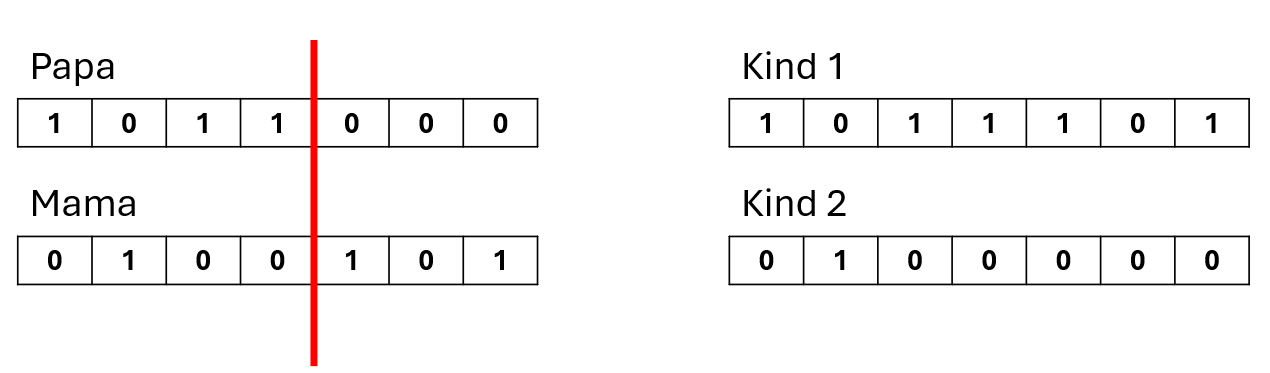
\includegraphics[width=0.8\textwidth]{
		papers/varalg/images/teil3/05GeneticStringCross.png
	}
	\caption{Ein einfaches Beispiel für eine Einpunkt-Kreuzung}
	\label{fig:one_point_crossover}
\end{figure}
Für die Kreuzung gibt es unterschiedliche Methoden, die gebräuchlichsten sind
die folgenden:
\begin{itemize}
	\item \textbf{Einpunkt-Kreuzung:} Ein zufälliger Punkt \( k \) \((1 \leq k < n)\)
\index{Einpunkt-Kreuzung}%
	wird auf den Elternchromosomen ausgewählt. Der Teil vor diesem Punkt stammt
	von einem Elternteil, die Gene ab diesem Punkt kommen vom anderen Elternteil. 
	Für die Erzeugung der Nachkommen wird mit den Formeln
	\begin{align*}
		O_1 = (P_1[1], P_1[2], \ldots, P_1[k], P_2[k+1], \ldots, P_2[n])\\
		O_2 = (P_2[1], P_2[2], \ldots, P_2[k], P_1[k+1], \ldots, P_1[n])
	\end{align*}
	gearbeitet. Die Abbildung \ref{fig:one_point_crossover} stellt diese Kreuzung bildlich dar.
	\item \textbf{Zweipunkt-Kreuzung:} Zwei zufällige Punkte \( k_1 \) und \( k_2 \)
\index{Zweipunkt-Kreuzung}%
	\((1 \leq k_1 < k_2 < n)\) werden ausgewählt und
	der Genabschnitt zwischen diesen Punkten wird zwischen den Eltern 
	getauscht. Die Nachkommen werden durch die Formeln
	\begin{align*}
		O_1 = (P_1[1], \ldots, P_1[k_1], P_2[k_1+1], \ldots, P_2[k_2], P_1[k_2+1], \ldots, P_1[n])\\
		O_2 = (P_2[1], \ldots, P_2[k_1], P_1[k_1+1], \ldots, P_1[k_2], P_2[k_2+1], \ldots, P_2[n])
	\end{align*}
	erzeugt.
	\item \textbf{Uniforme Kreuzung:} Jedes Gen wird mit einer bestimmten
\index{Kreuzung, uniform}%
\index{uniforme Kreuzung}%
	Wahrscheinlichkeit vom ersten oder zweiten Elternteil übernommen, was zu
	einer zufälligeren Kombination führt. Für jedes Gen \( i \) \((1 \leq i \leq n)\)
	wird eine zufällige Zahl \( r_i \) im Intervall [0, 1] gewählt. Wenn
	\( r_i \) kleiner als die vordefinierte Wahrscheinlichkeit \( p \) ist,
	dann wird das Gen von \( P_1 \) übernommen, ansonsten von \( P_2 \). Es
	wird über jede Position mit der Formel 
	\begin{align*}
		O_1[i] &=
		\begin{cases} 
			P_1[i] & \text{wenn } r_i < p       \\
			P_2[i] & \text{wenn } r_i \geq p 
		\end{cases}
		\\
		O_2[i] &=
		\begin{cases} 
			P_2[i] & \text{wenn } r_i < p       \\
			P_1[i] & \text{wenn } r_i \geq p 
		\end{cases}
	\end{align*}
	iteriert.
% 	Wissenstand der Leser ist vorausgesetzt
%	\footnote{
%		Iterieren wird typischerweise in der Informatik verwendet und 
%		bedeutet, dass über eine Menge der Reihe nach durchgegangen wird. 
%		Bei der Iteration über einen String wird jede Position des Strings 
%		angeschaut und je nach Aufgabe etwas mit diesem Zeichen gemacht.
%		}.
\end{itemize}

\subsubsection{Kreuzung auf das TSP angepasst
\label{buch:paper:varalg:subsection:crossover_tsp}}
Für das Travelling-Salesman-Problem muss der Algorithmus angepasst werden.
Würde das System wie in der Abbildung \ref{fig:one_point_crossover} 
übernommen werden, würde das Resultat unkorrekte Teile enthalten, was zu einem 
String wie in der Abbildung \ref{fig:one_point_crossover_cities} führt.
\begin{figure}
	\centering
	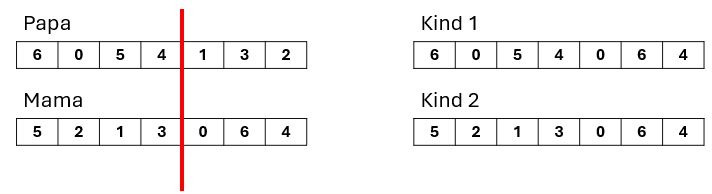
\includegraphics[width=0.8\textwidth]{
		papers/varalg/images/teil3/07GeneticStringCitiesCrossoverStandard.png
	}
	\caption{Beispiel einer Einpunkt-Kreuzung mit Städten ohne Anpassungen.}
	\label{fig:one_point_crossover_cities}
\end{figure}
Daher wird der Algorithmus so angepasst, dass keine Städte verschwinden
oder doppelte auftreten. Die einfachste Methode ist es, den Teil, der ersetzt wird,
zu entfernen und danach die fehlenden Teile nach der Reihenfolge des anderen
Elternteils zu ergänzen, bis der String wieder vollständig ist. Ein visuelles Beispiel
finden Sie in der Abbildung \ref{fig:crossover_order_cities}.
\begin{figure}
	\centering
	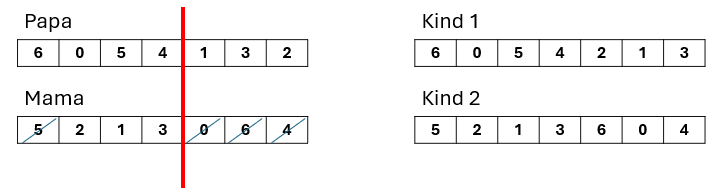
\includegraphics[width=0.8\textwidth]{
		papers/varalg/images/teil3/08GeneticStringCitiesCrossoverSimple.png
	}
	\caption{
		Beispiel einer Einpunkt-Kreuzung, welche angepasst an das TSP ist. Der ersetzende Teil wurde entfernt und
		nach der Reihenfolge des anderen Elternteils ergänzt.
	}
	\label{fig:crossover_order_cities}
\end{figure}
